\chapter{Lineær Programmering}
\textbf{Fokuspunkt: sammenskrivning af de to versioner}
Lineær programmering er en anvendelse af lineær algebra til at løse et optimeringsproblem. Lineære programmeringsproblemer tager udgangspunkt i maksimering eller minimering af en lineær funktion. For variablene er der fastsat en række af betingelser, som begrænser de mulige løsninger til problemet.
%Ved ikke: Må vi antage at læseren ved, hvad en lineær funktion er, for tror de ikke bare at det er ax +b?


Funktionen, som ønskes optimeret, kaldes \textbf{objektfunktionen}, og findes på formen:
\begin{align}
f(\vec{x})\ = \vec{c}^T \vec{x} \ =  c_1x_1 + c_2x_2 + \cdots + c_nx_n,
\end{align}
hvor $\vec{x}= \rvect{x_1 & x_2 & \cdots & x_n}^T$ og $\vec{c}= \rvect{c_1 & c_2 & \cdots & c_n}^T$.

\begin{comment}
Bør muligvis være en defintion, behøver ikke at skrives ud, men så skal f(\vec{x}) frem for f(x_1, ..., x_n).  Men det er jo variable repræcenteret ved en vektor så måske introducerer f(x_1, ..., x_n), udenfor definitionen.
\begin{defn}
Betragt et lineært programmerings problem, da er \textbf{objektfunktionen}
\begin{align*}
f(\vec{x}) = \vec{c}^T \cdot \vec{x}, 
\end{align*}
for $\vec{x}, \vec{c} \in \mathds{R}^n$, funktionen, som ønskes optimeret.
\end{defn} Eller noget, det er vigtigt at denne definition, vil kræve at vektor x og c bliver introduceret i den bindende tekst.
\end{comment}


%hvis objektfunktionen defineres, så bør det samme ske for bibetingelserne.
Dertil tilføjes en række af betingelser for variablene. Betingelser på formen
\begin{align}
	x_i \geq 0,
\end{align}
kaldes \textbf{positivitetsbetingelser}.
Andre lineære betingelser for variablene kaldes for \textbf{lineære bibetingelser}, og findes på formen, 
\begin{align}
	a_{i,1} x_1 + a_{i,2} x_2 + \cdots + a_{i,n} x_n \  = \ \vec{a}_i^T\vec{x} \ (\leq,=,\geq) \  b_i, \quad \text{for} \ i \in \{1,2,\cdots, m\}, %Kan man bruge \leq,=,\geq)?
\end{align}
hvor $m$ er antallet af lineære bibetingelser. I en lineær bibetingelse kan venstresiden være begrænset med $\leq, \geq$ eller $=$ i forhold til højresiden. I nogle typer af programmeringsproblemer anvendes kun en enkelt af disse relationer. Positivitetsbetingelser er et specialtilfælde af de lineære bibetingelser, da en positivitetsbetingelse, $x_i \geq 0$, blot kan ses som en lineær bibetingelse, hvor en koefficienten til $x_i$ er 1, mens resten af koefficienterne er 0 og hvor $b_i=0$.

En \textbf{mulig løsning} er en vektor $\vec{x}$, som overholder alle problemets betingelser. %Bør nok skrives som en definition, men det kan være at det først skal ske under geo? Bertimaz har i hvertfald en strangent def.

Et eksempel på et lineært programmeringsproblem ses i Eksempel \ref{eks:maksprob1}. Eksemplet er et lineært maksimeringsproblem, da objektfunktionen ønskes maksimeret.

\begin{eks}
Et eksempel på et lineært programmeringsproblem ses her, hvor funktionen $f(x_1,x_2)=4x_1+3 x_2$ skal maksimeres.
\begin{center}
\begin{tabular}{l	>{$}r<{$}	>{$}r<{$}	>{$}l<{$}}
Maksimer 		& 		4x_1&	+3 x_2	& \\
med hensyn til 	&  \ \ 	2 x_1& 	- 4 x_2	& \geq - 8\\
				&  		x_1& 	+3 x_2	& \leq 16\\
				&  \ \ 	x_1& 			& \leq 10\\
og $x_1,x_2\geq 0$
\end{tabular}
\end{center}


%Mængden af alle mulige løsninger til problemet kan vises grafisk. De mulige løsninger findes inden for det grå område på Figur \ref{fig:maksprob1}, hvor $x_1$ og $x_2$ vises henholdsvis på 1. og 2. aksen. %Hvor får du det grå område fra?
%
%\begin{center}
%	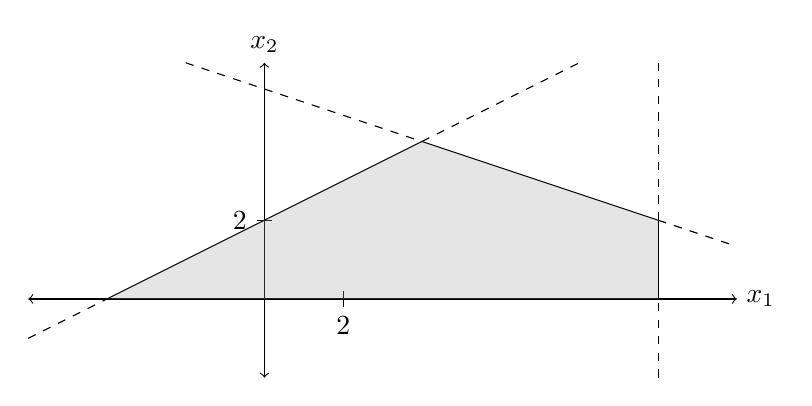
\begin{tikzpicture}
  %laver Grid
  	%\draw[thin,gray!40] (-3,-1) grid (6,3); 
  %x-aksen
  	\draw[<->] (-3,0)--(6,0) node[right]{$x_1$}; 
  %y-aksen
  	\draw[<->] (0,-1)--(0,3) node[above]{$x_2$};
  	
  %akse-markeringer
  	%\node[left] (xakse) at (0,1) {2};
  	\draw[] (-0.1,1) -- (0.1,1) node[pos=0,left] {2};
  	\draw[] (1,-0.1) -- (1,0.1) node[pos=0,below] {2};
  	
  %ligning 1
	\draw[domain=-3:-2,variable=\x,dashed] 	plot({\x},{0.5*\x+1});
	\draw[domain=-2:2,variable=\x] 			plot({\x},{0.5*\x+1});
	\draw[domain=2:4,variable=\x,dashed] 	plot({\x},{0.5*\x+1});
	
  %ligning 2
  	\draw[domain=-1:2,variable=\x,dashed] 	plot({\x},{-(1/3)*\x+8/3});
	\draw[domain=2:5,variable=\x] 			plot({\x},{-(1/3)*\x+8/3});
	\draw[domain=5:6,variable=\x,dashed] 	plot({\x},{-(1/3)*\x+8/3});
	

  %ligning 3
  	\draw[domain=-1:0,variable=\y,dashed] 	plot({5},{\y});
	\draw[domain=0:1,variable=\y] 			plot({5},{\y});
	\draw[domain=1:3,variable=\y,dashed] 	plot({5},{\y});

  %løsningsmængden skraveret
	\fill[gray!80,nearly transparent] (-2,0) -- (2,2) -- (5,1) --(5,0) --  cycle;
\end{tikzpicture}
%	\captionof{figure}{Grafisk repræsentation af mulige løsninger.}
%	\label{fig:maksprob1}
%\end{center} 

\label{eks:maksprob1}
\end{eks}

%%%%%%%%%%%%%%%%%%%%%%%%%%%%%%%%%%%%%%%%%%%%%%%%%%%%%%%%%%%%%%%%%%%%%%%%%%%%%%%%%%%%%%%%%%%%%%%%%%%%
%%%%%%%%%%%%%%%%%%%%%%%%%%%%%%%%%%%%%%%%%%%%%%%%%%%%%%%%%%%%%%%%%%%%%%%%%%%%%%%%%%%%%%%%%%%%%%%%%%%%%
Lineær programmering er en anvendelse af lineær algebra til at løse et optimeringsproblem. Lineære programmeringsproblemer tager udgangspunkt i maksimering eller minimering af en lineær funktion.
\begin{defn}[Lineær funktion]
Lad $f:\mathds{R} \to \mathds{R}$ være en funktion, da siges $f$ at være \textbf{lineær} hvis
\begin{enumerate}[label=\alph*]
\item $f(x_1 + x_2) = f(x_1) + f(x_2), \qquad \forall x_1,x_2 \in \mathds{R}$
\item $f(c\cdot x) = c \cdot f(x), \qquad \forall a, x \in \mathds{R}$
\end{enumerate}
\label{def:linfunk}
\end{defn}
Bemærk at selv om $f(x) = ax + b$ er kendt som en lineær funktion, er den ikke lineær pr Definition \ref{def:linfunk}.
Funktionen som skal optimeres kaldes objektfunktionen.
\begin{defn}
Betragt et lineært programmerings problem, da er \textbf{objektfunktionen}
\begin{align*}
f(\vec{x}) = \vec{c}^T \cdot \vec{x}, 
\end{align*}
for $\vec{x}, \vec{c} \in \mathds{R}^n$, funktionen, som ønskes optimeret.
\end{defn}
Objektfunktionen er repræsenteret som prikproduktet af en vektor $\vec{c}= \rvect{c_1 & c_2 & \cdots & c_n}^T$, der indeholder alle koefficienterne i funktionen og en vektor $\vec{x}= \rvect{x_1 & x_2 & \cdots & x_n}^T$, hvis indgange er funktionens variable.
Til objektfunktionen knyttes nogle bibetingelser, som variablene skal overholde. 
\begin{defn}[bibetingelser]
Lad $\vec{x}\in \mathds{R}$ repræsentere variabelene til et lineært programmeringsproblem, og $x_i$ for den $i$ indgang i $\vec{x}$ da kaldes betingelser på formen
\begin{enumerate}
\item \textbf{positivitetsbetingelser}: $x_i \geq 0$
\item \textbf{lighedsbetingelser}: $\vec{a}_i^T\vec{x} = b_i$
\item \textbf{størreendbetingelser}: $\vec{a}_i^T\vec{x} \geq b_i$
\item \textbf{mindreendbetingelser}: $\vec{a}_i^T\vec{x} \leq b_i$
\end{enumerate}
for $\vec{a_i}\in \mathds{R}^n$ og $b_i\in \mathds{R}$. 
Er $x_i$ ikke betinget af en positivitetsbetingelse kaldes den for en \textbf{frivariable}.
\end{defn}
Her betegner vektoren $\vec{a_i}$ koefficienterne i den $i$ bibetingelse, bemærk at hvis en ligning ikke indeholder den $j$ variable, da vil den $j$te indgang i koefficientvektoren $\vec{a_i}$ være lig nul, da der skal være en indgang pr variabel, ellers er prikproduktet ikke defineret. 

\section{Standard maksimerings- og minimeringsproblemer}
I et standard maksimeringsproblem gælder det, for alle bibetingelserne, at den lineære funktion af variablene er mindre end eller lig med en konstant.
Samtidig skal de i et standard minimeringsproblem være større end eller lig med en konstant. 
For begge problemer er variablene positivt begrænsede. 

Som beskrevet i Appendix \ref{afsnit:lign_sys} kan et lineært ligningssystem opskrives som et matrix-vektor produkt. 
Matricen repræsenterer koefficienterne i det lineære ligningssytem, mens variablene skrives som en vektor.
Tilsvarende gælder det for objektfunktionen, at denne kan skrives som et produkt af to vektorer. 
Dette tillader definitionen af et standard maksimeringsproblem med disse produkter i Definition \ref{def:std_maksmin}. 

\begin{defn}[Standard maksimering- og minimeringsproblemer]
	Lad $\vec{x}= \rvect{x_1 & x_2 & \cdots & x_n}^T$ være \textbf{løsningsvektoren} med koefficienter $\vec{c}= \rvect{c_1 & c_2 & \cdots & c_n}^T$ i objektfunktionen.
	Lad $A$ være en $m \times n$ matrix og lad $\vec{b}=\rvect{b_1 & b_2 & \cdots & b_m}^T$.\\
Da er standard maksimeringsproblemet defineret som
\begin{center}
\begin{tabular}{l	>{$}l<{$}}
Maksimer 		& \vec{c}^T\vec{x} \\
med hensyn til 	& A\vec{x} \leq \vec{b}\\
og 				& \vec{x} \geq \vec{0},
\end{tabular}
\end{center}
og standard minimeringsproblemet er defineret som
\begin{center}
\begin{tabular}{l	>{$}l<{$}}
Minimer			& \vec{c}^T\vec{x} \\
med hensyn til 	& A\vec{x} \geq \vec{b}\\
og 				& \vec{x} \geq \vec{0}.
\end{tabular}
\end{center}
\label{def:std_maksmin}
\end{defn}
Består ligningssystemet af ligheder, kaldes problemet henholdvist enten et \textbf{standard maksimeringsproblem med ligheder}, eller et \textbf{standard minimeringsproblem med ligheder}. \\

\begin{eks}[Standard maksimeringsproblem]
Hvis eksempel \ref{eks:maksprob1} skal omskrives til et standard maksimeringsproblem, skal alle  bibetingelserne være mindreendbetingelser.
Bibetingelse nr. 3 skal derved omskrives. Dette gøres ved at multiplicere begge sider af uligheden med $-1$, da dette vender ulighedstegnet. Derved bliver Eksempel \ref{eks:maksprob1} omskrevet til et standard maksimeringsproblem.
\begin{center}
\begin{tabular}{l	>{$}r<{$}	>{$}r<{$}	>{$}l<{$}}
Maksimer 		& 		4x_1	&	+3 x_2	& \\
med hensyn til 	&  \ \ 	-2 x_1	& 	+4 x_2	& \leq 8\\
				&  		x_1		& 	+3 x_2	& \leq 16\\
				&  \ \ 	x_1		& 			& \leq 10\\
og $x_1 \geq 0, x_2\geq 0$.
\end{tabular}
\end{center}
\label{eks:maksprob2}
\end{eks}

Bemærk, at på samme måde som bibetingelserne kan omskrives, kan et minimeringsproblem ligeledes laves til et maksimeringsproblem, ved at multiplicere med $-1$.



\begin{comment}
\begin{defn}[Standard minimum problem]
	Lad $\vec{x}= [x_1, x_2,\cdots, x_n]^T$ være \textbf{løsningsvektoren}, med koefficienter $\vec{c}= [c_1, c_2,\cdots, c_n]^T$ i objektfunktionen, og lad $m \times n$ matrixen $A=[A_{ij}]$ for $i=1,2,\cdots,m$ og $j=1,2,\cdots,n$ være begrænset af konstanterne $\vec{b}=[b_1, b_2,\cdots, b_m]^T$.
	Da er standard minimum problemet defineret som\\
\begin{center}
\begin{tabular}{l	>{$}l<{$}}
Minimer			& \vec{c}^T\vec{x} \\
med hensyn til 	& A\vec{x} \geq \vec{b}\\
og 				& \vec{x} \geq \vec{0}
\end{tabular}
\end{center}
\label{def:std_min}
\end{defn} %Hvorfor byttes der rundt på b og c? i min og max?


%%%%%%%%%%%%%%%%%%%%%%%%%%%%%%%%%%%%%%%%%%%%%%%%%%%%%%%%%%%%%%%%%%%%%%%%%%%%%%%%%%%%%%%%%%%%%%%%%%%%%%%%
%%%%%%%%%%%%%%%%%%%%%%%%%%%%%%%%%%%%%%%%%%%%%%%%%%%%%%%%%%%%%%%%%%%%%%%%%%%%%%%%%%%%%%%%%%%%%%%%%%%%%%%%%%

Det betyder at ethvert lineært programmeringsproblem kan omskrives, så det står på standardform.
\begin{defn}[Standard minimumsproblemer]
Lad $f(\vec{x}) = \vec{c}^T\vec{x}$ betegne objektfunktionen til et lineært minimeringsproblem, for $\vec{x},\vec{c} \in\mathds{R}^n$, lad $m \times n$ matricen $A=[A_{ij}]$ for $i=1,...,m$ og $j=1,...,n$, og lad $\vec{b} \in  \mathds{R}^n$.
Der er standard minimumsproblemet defineret som\\
\begin{center}
\begin{tabular}{l	>{$}l<{$}}
Minimer			& \vec{c}^T\vec{x} \\
med hensyn til 	& A\vec{x} \geq \vec{b}\\
og 				& \vec{x} \geq \vec{0}.
\end{tabular}
\end{center}
Består ligningssystemet af ligheder kaldes problemet; \textbf{standard minimumsproblem med ligheder}.
\label{def:std_maksmin}
\end{defn}
Bemærk at på samme måde som bibetingelserne kan omskrives, kan et minimeringsproblem laves til et maksimeringsproblem ved at multiplicere med $-1$, hvorfor at alle definitioner og sætninger er ækvivalente. Derfor defineres begreber og sætninger kun for minimums problemer, mens eksemplerne illustrere maksimums problemer.
\end{comment}
\subsection{Omskrivning mellem ligheder og uligheder}
Da et programmeringsproblem ikke nødvendigvis er på den ønskede form fra start af, er det vigtigt at kunne omskrive mellem uligheder og ligheder.\\
\begin{itemize}
\item Omskrivning mellem uligheder %Det er blevet bedere, men er stadig ikke helt godt
\begin{align*}
	\vec{a}_i^T\vec{x} \geq b_i \quad \Leftrightarrow \quad -\vec{a}_i^T\vec{x} \leq -b_i
\end{align*}
\item Omskrivning fra lighed til ulighed % hvorfor bruges der forskellige pile. rettet
\begin{center}
\begin{tabular}{>{$}l<{$} >{$}r<{$}}
	\vec{a}_i^T\vec{x} = b_i \quad \Leftrightarrow \quad 	& 
	\vec{a}_i^T\vec{x} \leq b_i \quad \text{og} \quad  \vec{a}_i^T\vec{x} \geq b_i \\ %Ved ikke om det vil give mening at have dem på samme linje og bruge \wedge i stedet for og.
\end{tabular}
\end{center}
\item Omskrivning fra ulighed til lighed\\
En ulighed kan omskrives til en lighed ved indførslen af en ikke-negativ \textbf{slack-variabel}, som udgør forskellen mellem $\vec{a}_i^T\vec{x}$ og $b_i$ i uligheden. 
Slack-variablen indgår kun i denne række af koefficientmatricen og får koefficient $1$ eller $-1$ afhængigt af uligheden i bibetingelsen.%, hvis uligheden  For maksimeringsproblemer får variabellen en koefficient på 1 i koefficientmatricen og -1 for minimeringsproblemer.
%Et standard maksimeringsproblem kan derved omskrives til ligheder ved at indføre en slackvariabel $x_{n+i}$ for hver bibetingelse. 
\begin{center}
\begin{tabular}{ >{$}l<{$} >{$}l<{$} >{$}l<{$}}
	\vec{a}_i^T \vec{x}  \leq b_i & \Rightarrow & \vec{a}_i^T \vec{x} \ + \ x_{n+i} \ = b_i\\
	\vec{a}_i^T \vec{x}  \geq b_i & \Rightarrow & \vec{a}_i^T \vec{x} \ -\ x_{n+i} \ = b_i
\end{tabular} %Du skriver at du gør det for max, men du gør det også for min.
\end{center} % Itemmize fungere okay, for de to første men dette afsnit bliver for langt til at det kan være et punkt, i min optik.

\begin{comment}
Derved bliver betingelserne for henholdsvis et maksimeringsproblem og et minimeringsproblem omskrevet til:
\begin{align*}
	A' &=\rvect{A & I_m}\\
	A' &=\rvect{A & -I_m}
\end{align*}

\end{comment}
%Nok en god idet at komme med et eksemple så \vec{a_i} \vec{x} + x_{n+i} = b_i indflettet, på lige fod med for omskrivning af mellem uligheder.
\end{itemize}



\begin{eks}[Standard maksimumsproblem]
Hvis eksempel \ref{eks:maksprob1} skal omskrives til et standard maksimumsproblem, skal alle relationer i bibetingelserne være $\leq$. %pas på med matematiske tegn i bindende tekst.
Bibetingelse nr. 3 skal derved omskrives. Dette kan gøres ved at multiplicere begge sider af uligheden med $-1$, da dette vender ulighedstegnet. Derved bliver Eksempel \ref{eks:maksprob1} omskrevet til et standard maksimumsproblem.\\
\begin{center}
\begin{tabular}{l	>{$}r<{$}	>{$}r<{$}	>{$}l<{$}}
Maksimer 		& 		4x_1	&	+3 x_2	& \\
med hensyn til 	&  \ \ 	-2 x_1	& 	+4 x_2	& \leq 8\\
				&  		x_1		& 	+3 x_2	& \leq 16\\
				&  \ \ 	x_1		& 			& \leq 10\\
og $x_1 \geq 0, x_2\geq 0$.
\end{tabular}
\end{center}
%Man må vel ikke bare sige at x_1 \geq 0, men man skal sige at x_1 = x_3 - x_4, hvor x_3, x_4 \geq 0.

%\begin{center}
%	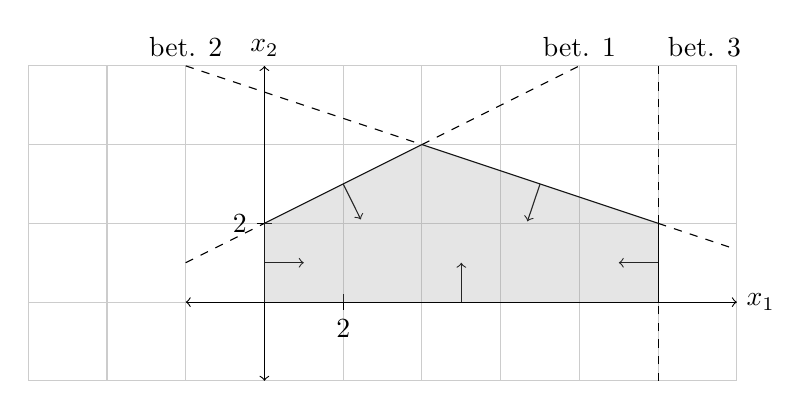
\begin{tikzpicture}
  %laver Grid. godt til når koordinater skal redigeres
  	\draw[thin,gray!40] (-3,-1) grid (6,3); 
  %x-aksen
  	\draw[<->] (-1,0)--(6,0) node[right]{$x_1$};
  	\draw[->] (2.5,0) -- (2.5,0.5);
  %y-aksen
  	\draw[<->] (0,-1)--(0,3) node[above]{$x_2$};
  	\draw[->] (0,0.5) -- (0.5,0.5);
  	
  %akse-markeringer
  	%\node[left] (xakse) at (0,1) {2};
  	\draw[] (-0.1,1) -- (0.1,1) node[pos=0,left] {2};
  	\draw[] (1,-0.1) -- (1,0.1) node[pos=0,below] {2};
  	
  %ligning 1
	\draw[domain=-1:0,variable=\x,dashed] 	plot({\x},{0.5*\x+1});
	\draw[domain=0:2,variable=\x] 			plot({\x},{0.5*\x+1});
	\draw[domain=2:4,variable=\x,dashed] 	plot({\x},{0.5*\x+1}) node[above] {bet. 1};
  	\draw[->] (1,1.5) -- (1.224,1.05);
	
  %ligning 2
  	\draw[domain=-1:2,variable=\x,dashed] 	plot({\x},{-(1/3)*\x+8/3}) node[above] at (-1,3) {bet. 2} ;
	\draw[domain=2:5,variable=\x] 			plot({\x},{-(1/3)*\x+8/3});
	\draw[domain=5:6,variable=\x,dashed] 	plot({\x},{-(1/3)*\x+8/3});
	\draw[->] (3.5,1.5) -- (3.34,1.026);

  %ligning 3
  	\draw[domain=-1:0,variable=\y,dashed] 	plot({5},{\y});
	\draw[domain=0:1,variable=\y] 			plot({5},{\y});
	\draw[domain=1:3,variable=\y,dashed] 	plot({5},{\y}) node[above right] {bet. 3};
	\draw[->] (5,0.5) -- (4.5,0.5);

  %løsningsmængden skraveret
	\fill[gray!80,nearly transparent] (0,0) -- (0,1) -- (2,2) -- (5,1) --(5,0) --  cycle;
\end{tikzpicture}
%	\captionof{figure}{Den mulige mængde af et standard maksimeringsproblem.}
%	\label{fig:maksprob2}
%\end{center}

\label{eks:maksprob2}
\end{eks}

%%%%%%%%%%%%%%%%%%%%%%%%%%%%%%%%%%%%%%%%%%%%%%%%%%%%%%%%%%%%%%%%%%%%%%%%%%%%%%%%%%%%%%%%%%%%%%
%%%%%%%%%%%%%%%%%%%%%%%%%%%%%%%%%%%%%%%%%%%%%%%%%%%%%%%%%%%%%%%%%%%%%%%%%%%%%%%%%%%%%%%%%%%%
Da bibetingelserne er ligninger repræsenteret ved et prikprodukt, kan hele ligningssystemet repræsenteres som et matrix-vektorprodukt, det kræver dog, at alle ikke positivitets betingelser er på samme form.
Det kan derfor være favorabelt at kunne omskrive fra en ulighed til en anden.
\begin{stn}
Lad $\vec{a}_i^T,\vec{x} \in \mathds{R}^n$ og $b_i \in \mathds{R}$, da gælder:
\begin{enumerate}
\item $\vec{a}_i^T\vec{x} \geq b_i \quad \Leftrightarrow \quad -\vec{a}_i^T\vec{x} \leq -b_i$
\item $\vec{a}_i^T\vec{x} = b_i \quad \Leftrightarrow  \quad  \vec{a}_i^T\vec{x} \leq b_i \quad \wedge \quad  \vec{a}_i^T\vec{x} \geq b_i$
\item $\vec{a}_i^T \vec{x}  \leq b_i \quad \Rightarrow \quad  \vec{a}_i^T \vec{x}  +  x_{n+i}  = b_i$
\item $\vec{a}_i^T \vec{x}  \geq b_i \quad \Rightarrow \quad  \vec{a}_i^T \vec{x}  - x_{n+i}  = b_i$
\end{enumerate}
hvor $x_{n+i}$ er en slack variable. 
\end{stn}
Dermed kan bibetingelserne skrives som $A\vec{x}\geq \vec{b}$, hvor $\vec{a_i}$ udgør den $i$te række i $A$ og $b_i$ er den $i$ indgang i $\vec{b}$.
Bemærk at positivitetsbetingelserne er et særtilfælde af størreendbetingelser, hvor en koefficienten til $x_i$ er 1, mens resten af koefficienterne er 0 og hvor $b_i=0$.
Positivitets betingelsen skrives ikke med i ligningssystemet, og i stedet er det som oftes underforstået, at enhver variable skal være ikke negativ.
For at det skal gøre sig gældende, skal en hver frivariable omskrives så de er betinget af en positivitetsbetingelse.
\begin{stn}
Lad $x_i$ være en frivariabel, da er $x_i = x_{n+i}-x_{n+i+1}$, hvor $x_{n+i},x_{n+i+1}\geq 0$.
\end{stn}
\section{Løsninger til linære programmeringsproblemer}

Den mulige mængde er mængden af løsningsvektorer, $\vec{x}$, som opfylder alle problemets betingelser. Hvis en optimal løsning eksisterer, vil denne derved være indeholdt i den mulige mængde.

\begin{defn}[Mulige løsninger og den mulige mængde]
En \textbf{mulig løsning} er en løsningsvektor $\vec{x}$, som opfylder alle problemets betingelser.\\
\textbf{Den mulige mængde} $\mathcal{F}$ er mængden af alle de mulige løsninger. Den vil derfor, for et standard maksimeringsproblem, være defineret som
\begin{align*}
\mathcal{F}=\{\vec{x} \in \mathds{R}^n|A\vec{x} \leq \vec{b}, \vec{x} \geq \vec{0}\}.
\end{align*}
Et problem kaldes \textbf{inkonsistent}  hvis den mulige mængde er den tomme mængde, ellers er problemet \textbf{konsistent}. 
\end{defn}

I lineær programmering søges der efter en optimal løsning, som vil være den mulige løsning, der enten maksimerer eller minimerer objektfunktionen, afhængig af, om der er tale om et maksimerings- eller minimeringsproblem. 
Husk på, at et maksimeringsproblem kan laves til et minimeringsproblem, hvorfor det kun er nødvendigt at definere den optimale løsningsværdi for minimeringsproblemet.
\begin{defn}[Optimal løsningsværdi]
Lad $f$ være objektfunktionen til et lineært minimeringsproblem, da kaldes en vektor $\vec{x}^*$ en \textbf{optimal løsningsværdi}, hvis 
\begin{align}
	f(\vec{x}^*)=\min\limits_{\vec{x} \in \mathcal{F}}f(\vec{x}).
\end{align}
Værdien af $f(\vec{x}^*)$ kaldes den \textbf{optimale værdi}.
\end{defn}

Den optimale løsning kan findes på forskellige måder, heriblandt med Simplex metoden, som beskrives i Kapitel \ref{chap:simp}. En anden måde er ved geometrisk visualisering af den mulige mængde. Denne metode er mulig for problemer med op til 3 variable, da løsningsmængden derved visualiseres som et plot i det tilsvarende antal dimensioner. De mulige løsninger findes således inden for det område, der er begrænset af betingelserne. 

\begin{eks}[Den mulige mængde]
Ved at indtegne betingelserne i et koordinatsystem er det muligt at visualisere den mulige mængde som fællesmængden af de mængder, der dannes ud fra betingelserne. På Figur \ref{fig:maksprob2} er den mulige mængde for problemet i Eksempel \ref{eks:maksprob2} indtegnet. Der er desuden tegnet en pil for hver betingelse, som viser, for hvilken side af linjen, koordinaterne opfylder betingelsen. Den mulige mængde er farvet grå.

\begin{center}
	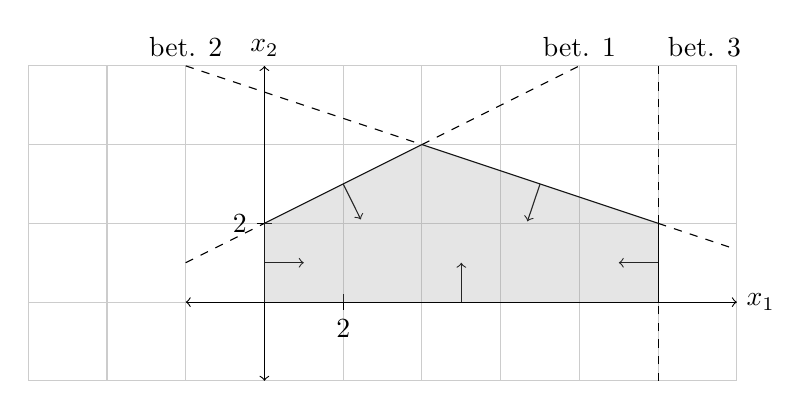
\begin{tikzpicture}
  %laver Grid. godt til når koordinater skal redigeres
  	\draw[thin,gray!40] (-3,-1) grid (6,3); 
  %x-aksen
  	\draw[<->] (-1,0)--(6,0) node[right]{$x_1$};
  	\draw[->] (2.5,0) -- (2.5,0.5);
  %y-aksen
  	\draw[<->] (0,-1)--(0,3) node[above]{$x_2$};
  	\draw[->] (0,0.5) -- (0.5,0.5);
  	
  %akse-markeringer
  	%\node[left] (xakse) at (0,1) {2};
  	\draw[] (-0.1,1) -- (0.1,1) node[pos=0,left] {2};
  	\draw[] (1,-0.1) -- (1,0.1) node[pos=0,below] {2};
  	
  %ligning 1
	\draw[domain=-1:0,variable=\x,dashed] 	plot({\x},{0.5*\x+1});
	\draw[domain=0:2,variable=\x] 			plot({\x},{0.5*\x+1});
	\draw[domain=2:4,variable=\x,dashed] 	plot({\x},{0.5*\x+1}) node[above] {bet. 1};
  	\draw[->] (1,1.5) -- (1.224,1.05);
	
  %ligning 2
  	\draw[domain=-1:2,variable=\x,dashed] 	plot({\x},{-(1/3)*\x+8/3}) node[above] at (-1,3) {bet. 2} ;
	\draw[domain=2:5,variable=\x] 			plot({\x},{-(1/3)*\x+8/3});
	\draw[domain=5:6,variable=\x,dashed] 	plot({\x},{-(1/3)*\x+8/3});
	\draw[->] (3.5,1.5) -- (3.34,1.026);

  %ligning 3
  	\draw[domain=-1:0,variable=\y,dashed] 	plot({5},{\y});
	\draw[domain=0:1,variable=\y] 			plot({5},{\y});
	\draw[domain=1:3,variable=\y,dashed] 	plot({5},{\y}) node[above right] {bet. 3};
	\draw[->] (5,0.5) -- (4.5,0.5);

  %løsningsmængden skraveret
	\fill[gray!80,nearly transparent] (0,0) -- (0,1) -- (2,2) -- (5,1) --(5,0) --  cycle;
\end{tikzpicture}
	\captionof{figure}{Skravering af den mulige mængde for et standard maksimeringsproblem.}
	\label{fig:maksprob2}
\end{center}
\end{eks}

Løsningerne til et optimeringsproblem er beskrevet som værende alle de vektorer, $\vec{x}$, som overholder bibetingelserne. Løsningsmængden til bibetingelserne er beskrevet som et polyeder.
\begin{defn} [Polyeder]
Et \textbf{Polyeder} er en mængde 
\begin{align*}
 P =\{ \vec{x} \in \mathds{R}^n | A \vec{x} \geq \vec{b}, \vec{b}\in \mathds{R}^m\},
\end{align*}
hvor $A$ er en $m \times n$ matrix.
\end{defn}
Hvis et lineært programmeringsproblem står på standardform med ligheder $\{ \vec{x} \in \mathds{R}^n | A \vec{x} = \vec{b}, \vec{b}\in \mathds{R}^m\}$, så kaldes det stadig et polyeder.\\
Hvis der er et polyeder $P=\{\vec{x} \in \mathds{R}\mid A\vec{x}=\vec{b},\vec{x}\geq \vec{0}\}$, som består af alle bibetingelserne for problemet, så må der også findes et andet polyeder $Q$, som består af alle de lineært uafhængige bibetingelser for problemet. Da $P$ består af de samme bibetingelser som $Q$ og lidt flere til, så er en løsning $\vec{x}$ til $P$ nødvendigvis også en løsning til $Q$, og modsat er en løsning til $Q$ også en løsning til $P$. Derfor må $Q=P$, hvilket vil blive vist i følgende sætning.

\begin{stn}[Q=P]
Lad $P=\{\vec{x} \in \mathds{R}^n\mid A\vec{x}=\vec{b},\vec{x}\geq \vec{0}\}$ være et ikke-tomt polyeder, hvor $A$ er en $m\times n$ matrix.\\
Antag at $rang(A)=k<m$ og at rækkerne $\vec{a_i}^T$ for $i=1,\dots ,k$ er lineært uafhængig. Betragt polyederet $Q=\{\vec{x} \in \mathds{R}^n\mid \vec{a_i}^T\vec{x}=b_{i}, \vec{x}\geq \vec{0}, i = 1,\dots	k\}$. Så er $Q=P$.
\label{stn:PQ}
\end{stn}

\begin{proof}
Hvis $P=\{\vec{x} \in \mathds{R}^n\mid A\vec{x}=\vec{b}, \vec{x}\geq \vec{0}\}$ er et polyeder med $rang(A)=k$, afgrænset af alle bibetingelserne, så må der være et polyeder $Q=\{\vec{x} \in \mathds{R}^n\mid \vec{a_i}^T\vec{x}=b_{i}, \vec{x}\geq \vec{0}, i = 1,\dots,	k\}$, der består af alle lineært uafhængige bibetingelser. Så må $P\subseteq Q$, eftersom alle elementerne i $P$ også tilfredsstiller bibetingelserne for $Q$.\\
Eftersom $rang(A)=k$, så former rækkerne $\vec{a_1},\dots ,\vec{a_k}$ en basis for rækkerummet. Derfor kan enhver række $\vec{a}_j$ fra $A$ skrives som en linearkombination af de lineært uafhængige rækker $\vec{a}_i$ for $i = 1,...,k$.
Dermed bliver $\vec{a}_j = \sum_{i=1}^k c_{ij}\vec{a}_i$ for skalarer $c_{ij}$.

 Lad så $\vec{x}$ være en del af $P$ så
\begin{align*}
\vec{a}_j^T\vec{x}=\sum_{i=1}^{k}c_{i j}\vec{a}_i^T\vec{x}=\sum_{i=1}^{k}c_{i j}\vec{b}_i=\vec{b}_j, \qquad j=1,\dots,m.
\end{align*}
Derfor kan det konkluderes, at $P \subseteq Q$.\\
Lad nu $\vec{y}$ være en del af $Q$, så er $\vec{y}$ også en del af $P$, eftersom
\begin{align*}
\vec{a}_j^T\vec{y}=\sum_{i=1}^{k}c_{i j}\vec{a}_i^T\vec{y}=\sum_{i=1}^{k}c_{i j}\vec{b}_i=\vec{b}_j, \qquad j=1,\dots,m.
\end{align*}
Hvilket betyder, at $\vec{y}\in P$ og $Q\subseteq P$, og derved er $P=Q$.
\end{proof}

Derfor kan det antages, at alle bibetingelserne er lineært uafhængige uden at miste generelitet. 

%Et polyeder kan, alt efter bibetingelserne, være en mængde, der strækker sig ud i det uendelige, eller det kan være begrænset. 
%Hvis der er med et maksimeringsproblem at gøre, kan det ses, at bibetingelserne danner et område, men ved et minimeringsproblem, vil bibetingelserne ofte resultere i, at polyederet strækker sig ud i det uendelige, og derfor ikke længere er en form. Selvom dette er tilfældet, kaldes løsningsmængden stadig for et polyeder. \\
%Et problem kaldes \textbf{ubegrænset}, hvis objektfunktionen kan tage arbitrært store funktionsværdier for maksimeringsproblemer, og arbitrært små funktionsværdier for minimeringsproblemer. Ellers kaldes problemet \textbf{begrænset}.

%\begin{defn} [Begrænset]
%Lad $S \subset \mathds{R}^n$, da er $S$ begrænset, hvis der eksisterer en konstant $K$ så $\forall \vec{x} \in S: |\vec{x}| \leq K$.
%\end{defn}
%
%Med andre ord; hvis der findes en konstant, som er højere end den absolutte værdi af alle $\vec{x} \in S \in S$, og hvis der ikke eksisterer en konstant, som er støre end $|\vec{x}|$, så vil alle $\vec{x}$ gå mod uendeligt.

